\documentclass[12pt]{article}

\usepackage{graphicx}
\usepackage[margin=0.75in]{geometry}
\usepackage{multirow}

\usepackage{amsmath}
\usepackage{bm}
\newcommand{\m}[1]{\mathbf{\bm{#1}}}

\begin{document}

\section*{Homework 2 -- AMS 276}
\subsection*{Mickey Warner}
\bigskip
\bigskip

\section*{M1 -- Weibull baseline}

\noindent The likelihood for the proportionl hazards model with a Weibull as the baseline hazard function is given by
\[ L(\m{y}|\m{x},\m{\nu},\alpha,\gamma,\beta) = \prod_{\{i:\nu_i=1\}} \alpha\gamma y_i^{\alpha-1} \times \prod_{i=1}^n\exp\left[-\gamma y_i^\alpha e^{x_i^\top\beta}\right] \]
\noindent where for subject $i$, $y_i$ is the length of time in the study, $\nu_i$ is an indicator of whether a failure was observed, and $x_i$ is an indicator for the aneuploid group.
\bigskip

\noindent I place independent gamma priors on $\alpha,\gamma$ and a normal prior on $\beta$:
\begin{eqnarray*}
\alpha &\sim& Gamma(1, 0.1) \\
\gamma &\sim& Gamma(1, 0.1) \\
\beta &\sim& Normal(0, 10^2)
\end{eqnarray*}
\noindent The full conditional for the joint parameter vector $(\alpha, \gamma, \beta)$ is proportional to the likelihood times each of the priors:
\[ \pi(\alpha,\gamma,\beta|\m{y},\m{x},\m{\nu}) = \prod_{\{i:\nu_i=1\}} \alpha\gamma y_i^{\alpha-1} \times \prod_{i=1}^n\exp\left[-\gamma y_i^\alpha e^{x_i^\top\beta}\right]\times e^{-0.1\alpha}e^{-0.1\gamma}\exp\left(-\frac{\beta^2}{2\cdot10^2}\right) \]
\noindent The parameters are updated jointly using Metropolis-Hastings updates. Plots of their marginal posterior distributions and an estimate of the survival functions for the two groups (Aneuploid in blue and Diploid in red) are given at the end.
\bigskip

\noindent For this model, the survival function is computed by
\[ S(t|x,\alpha,\gamma,\beta)=\exp\left[-\gamma t^\alpha \exp\left(x\beta\right)\right]. \]

\section*{M2 -- Piece-wise constant}

\noindent We define a partion $0=s_0 < s_1 < \cdots < s_J$ by the quantiles of the failure times. We let $J=20$, with $s_j$ being the $(5\times j)$th quantile. Define $\delta_{ij}=1$ if $y_i\in(s_{j-1},s_j]$ and $0$ otherwise.
\bigskip

\noindent The likelihood for the piece-wise constant hazard model is given by
\[ L(\m{y}|\m{x},\m{\nu},\m{\lambda},\m{\beta}) = \prod_{i=1}^n\prod_{j=1}^J(\lambda_j e^{\m{x}_i^\top\m{\beta}})^{\delta_{ij}\nu_i}\exp\left(-\delta_{ij}\left[\lambda_j(y_i-s_{j-1})+\sum_{g=1}^{j-1}\lambda_g(s_g-s_{g-1})\right]e^{\m{x}_i^\top\m{\beta}}\right) \]
\noindent If $j=1$, then the summation in the exponent (which is for calculating the cumulative hazard function) becomes 0.
\bigskip

\noindent In this model we include an intercept term (described why later). For priors, we have
\begin{eqnarray*}
\lambda_k &\overset{iid}\sim& Gamma(1, 0.1),~~~~~k=1,\ldots,J \\
\beta_l &\overset{iid}\sim& Normal(0, 10^2),~~~~~l=0,1 \\
\end{eqnarray*}
\noindent 
\noindent The full posterior distribution is given by
\[ \pi(\m{\lambda}, \m{\beta}|\m{y},\m{x},\m{\nu}) \propto L(\m{y}|\m{x},\m{\nu},\m{\lambda},\m{\beta}) \prod_{k=1}^J p(\lambda_k) \prod_{l=0}^1 p(\beta_l) \]
\noindent We again update the parameters jointly, and I believe it is for this reason why it was necessary for me to include an intercept term. I don't fully understand it, but I would not get a correct answer if I exclude the intercept.
\bigskip

\noindent At time $s_j$, the survival function is computed by
\[ S(s_j|\m{x},\m{\lambda},\m{\beta})=\exp\left[-\exp\left(\m{x}^\top\m{\beta}\right)\sum_{g=1}^j\lambda_g(s_g-s_{g-1})\right]. \]

\section*{M3 -- Gamma process}

\noindent We use the same partition over the failure times as used in M2. We further define
\begin{eqnarray*}
    R_j &=& \{i:s_{j-1}<y_i\} \\
    D_j &=& \{i:s_{j-1}<y_i\leq s_j,\nu_i=1 \} \\
R_j-D_j &=& R_j \cap D_j^c
\end{eqnarray*}
\noindent We assume the baseline cumulative hazard function follows a gamma process, i.e. $H_0\sim GP(c_0 H^\star, c_0)$, where $c_0>0$ and $H^\star(t)>0$ is an increasing function. This implies the following prior for the jumps in the cumulative hazard
\[ h_j=H_0(s_j)-H_0(s_{j-1})\overset{ind}\sim Gamma(c_0(H^\star(s_j) - H^\star(s_{j-1})), c_0) \]

\noindent We use a grouped-data likelihood:
\begin{eqnarray*}
L(\m{y}|\m{x},\m{\nu},\m{h},\m{\beta}) &=& \prod_{j=1}^J G_j \\
&=& \prod_{j=1}^J\left\{\exp\left(-h_j\sum_{R_j-D_j}e^{\m{x}_i^\top\m{\beta}}\right)\prod_{D_j}\left[1-\exp(-h_j e^{\m{x}_i^\top\m{\beta}})\right]\right\}
\end{eqnarray*}
\noindent In the case of $D_j=\emptyset$ or $R_j-D_j=\emptyset$, the respective terms in the likelihood give no contribution. As in M2, we again include an intercept term.
\bigskip

\noindent $H^\star$ is chosen to be Weibull, so that $H^\star(t)=\gamma t^\alpha$. The priors we select are
\begin{eqnarray*}
\alpha  &\sim& Gamma(1, 1) \\
\gamma  &\sim& Gamma(1, 1) \\
\beta_0 &\sim& Normal(0, 10^2) \\
\beta_1 &\sim& Normal(0, 10^2) \\
c_0     &\sim& Gamma(1, 1)
\end{eqnarray*}
\noindent From M1, we don't expect $(\alpha, \gamma)$ in this case to be much different than around 1. Placing priors on $H^\star$ and $c_0$ should provide us with additional flexibility.
\bigskip

\noindent The full posterior is
\[ \pi(\m{h},\m{\beta},\alpha,\gamma,c_0|\m{y},\m{x},\m{\nu}) \prod_{j=1}^J \left[G_j \times p(h_j|\alpha, \gamma, c_0)\right] p(\alpha) p(\gamma) p(c_0) p(\beta_0) p(\beta_1) \]
\noindent We obtain posterior samples by alternating updates between two groups of parameters: $(\alpha,\gamma,\beta_0,\beta_1,c_0)$ and $\m{h}$. This is solely for mixing purposes; we use $\pi(\m{h},\m{\beta},\alpha,\gamma,c_0|\cdot)$ in both cases, as opposed to the full conditionals for these joint parameter vectors.
\bigskip

\noindent At time $s_j$ the survival function is calculated by
\[ S(s_j|\m{x},\m{h},\m{\beta})=\exp\left[-\exp\left(\m{x}^\top\m{\beta}\right)\sum_{g=1}^jh_g\right]. \]

\section*{Remarks about the posteriors and figures}

\noindent For the most part, there did not seem to be any issue with convergence in the posteriors. When such issues did arise, it was sufficient to increase the number of post-burn-in samples.
\bigskip

\noindent For each model, the posterior survival function for the two groups is given. The dashed lines are the same across the models, being the Kaplan-Meier estimates of $S$. The solid lines are from the posterior samples. The thicker lines are the means and the thinner are 95\% credible bands. In every case, our posterior estimates for the survival function seem to agree nicely with K-M. This may lead toward favoring M1, as it is the simplest.
\bigskip

\noindent For M1, density estimates and 95\% credible intervals are given for each of the three parameters. For M2, the distribution for $\beta_1$ is given (comparable to M1's $\beta$). Boxplots of the $J=20$ posterior hazards are shown. Since we had an intercept term, the parameters shown in the boxplot are not the $\lambda_j$'s, but rather $\lambda_j \exp(\beta_0)$, with the latter being the height of the hazard function at within $(s_{j-1},s_j]$. The figures for M3 are comparable to those in M2.
\bigskip

\noindent Overall, each model seems appropriate. M1 was far easier to implement than M2 and M3, but is not as robust. My main issue has been with the necessary inclusion of the intercept term $\beta_0$ for M2 and M3. I suspect it is because I did not update the parameters one at a time with their full conditionals, but I did not think that should have been an issue.


\newpage
\subsection*{Figures for M1}
\begin{center}
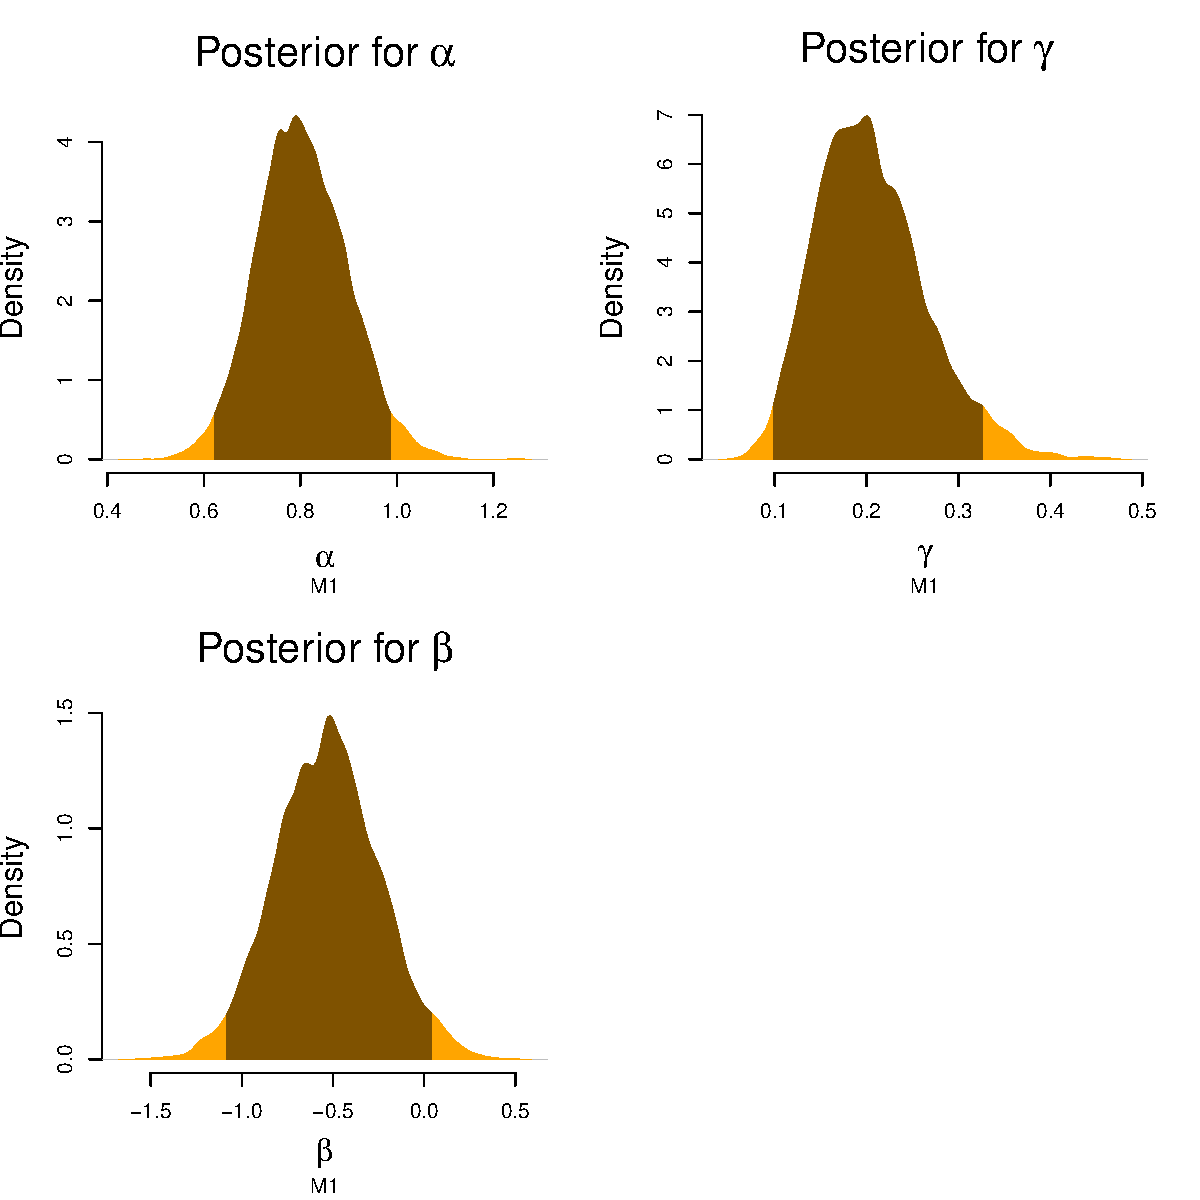
\includegraphics[scale=0.647]{figs/m1_post.pdf}
\bigskip
\bigskip

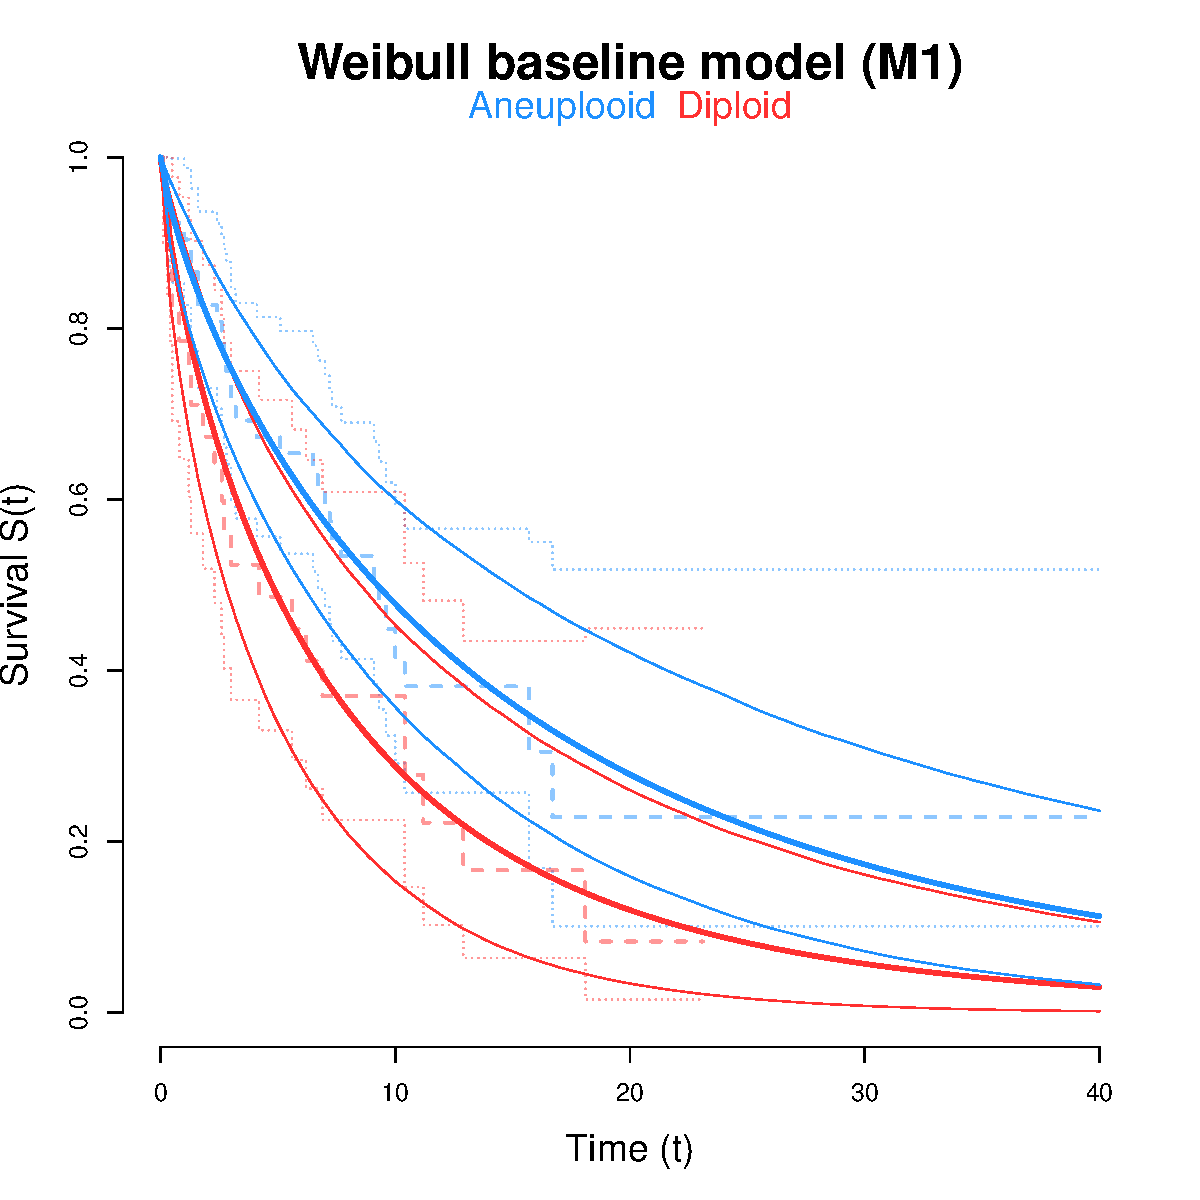
\includegraphics[scale=0.45]{figs/m1_surv.pdf}
\end{center}

\newpage
\subsection*{Figures for M2}
\begin{center}
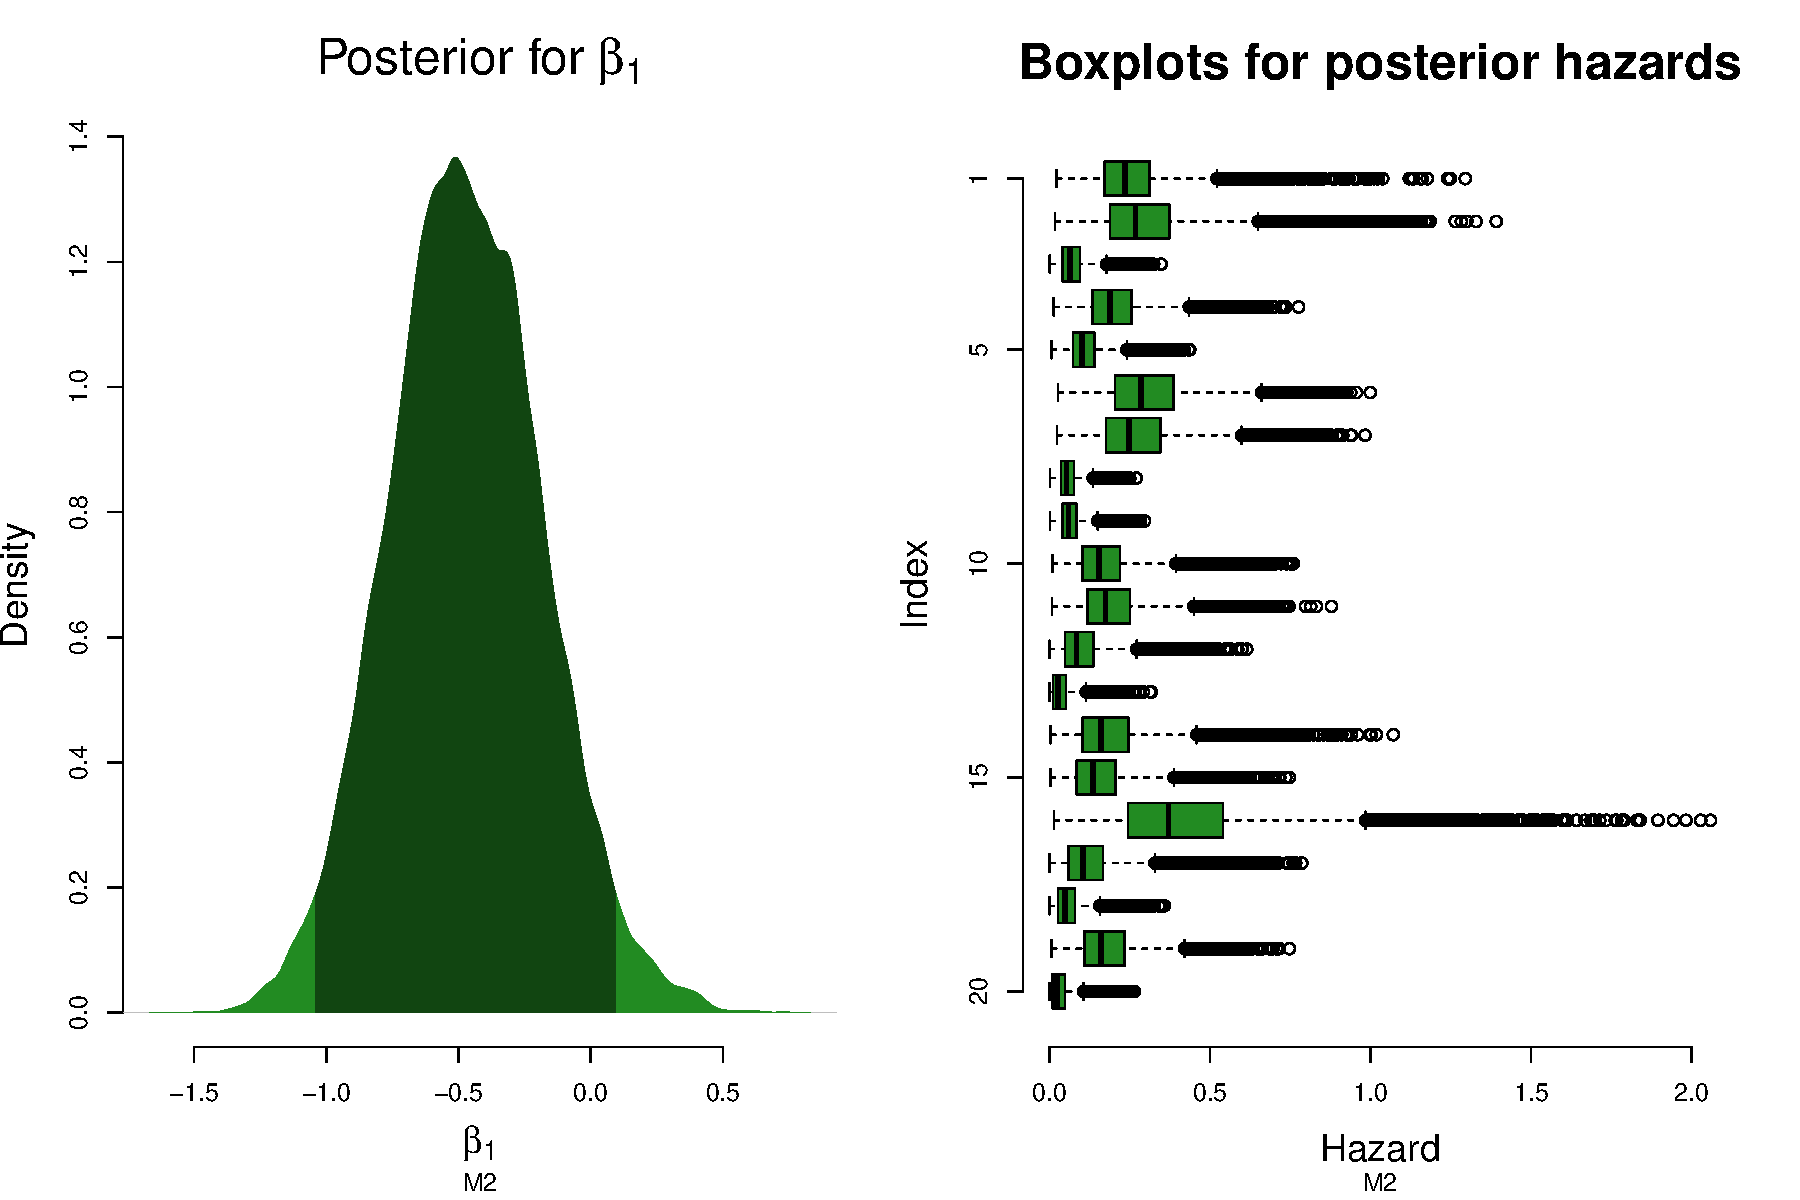
\includegraphics[scale=0.60]{figs/m2_post.pdf}
\bigskip
\bigskip

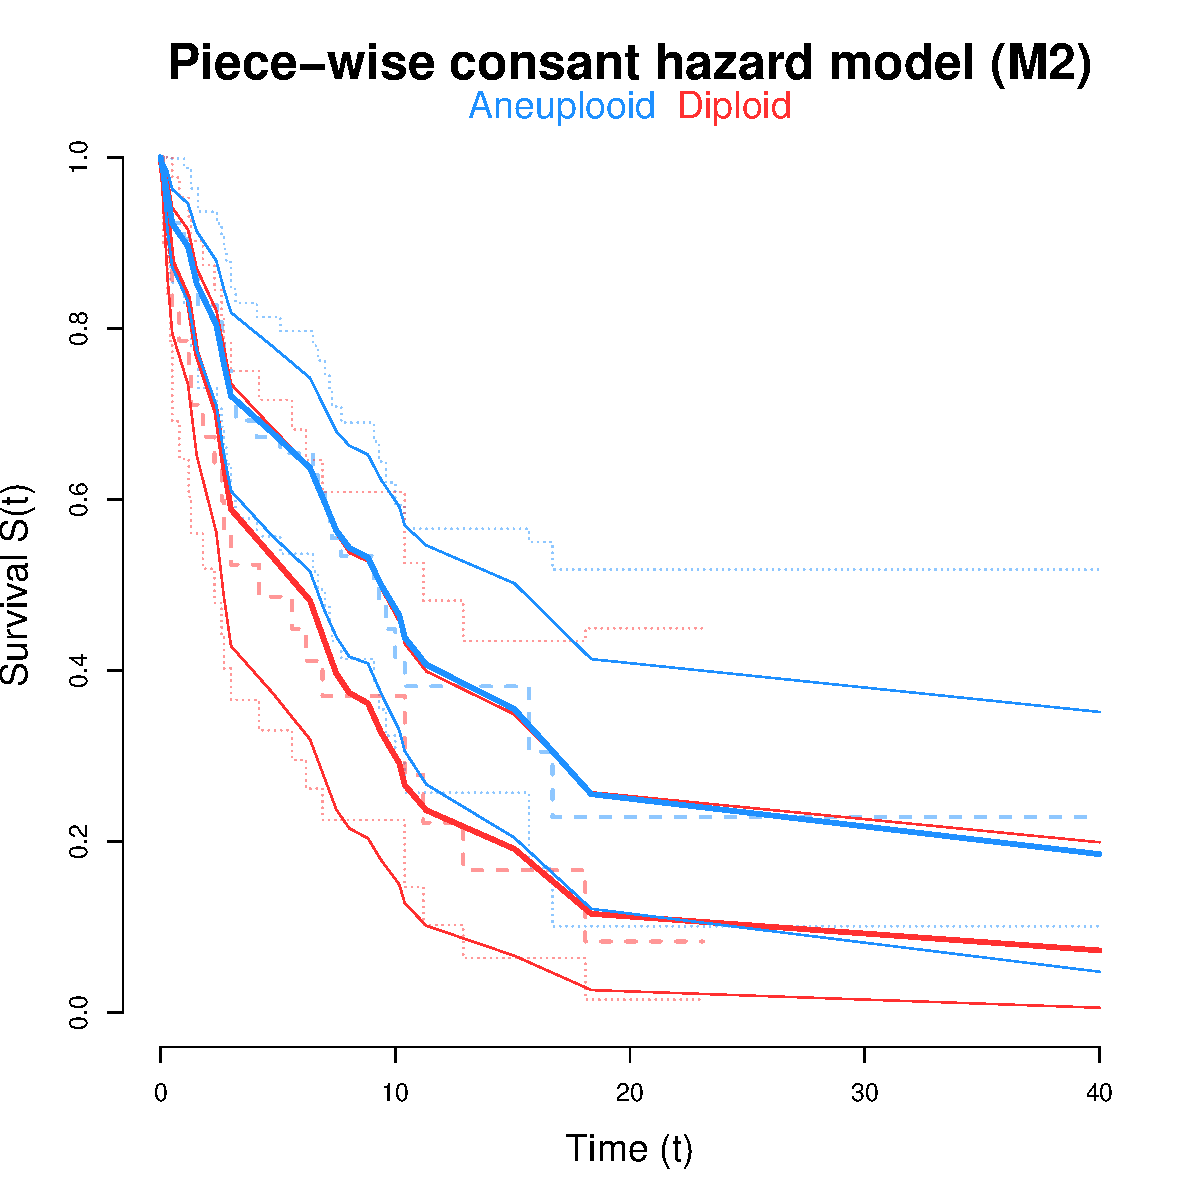
\includegraphics[scale=0.45]{figs/m2_surv.pdf}
\end{center}

\newpage
\subsection*{Figures for M3}
\begin{center}
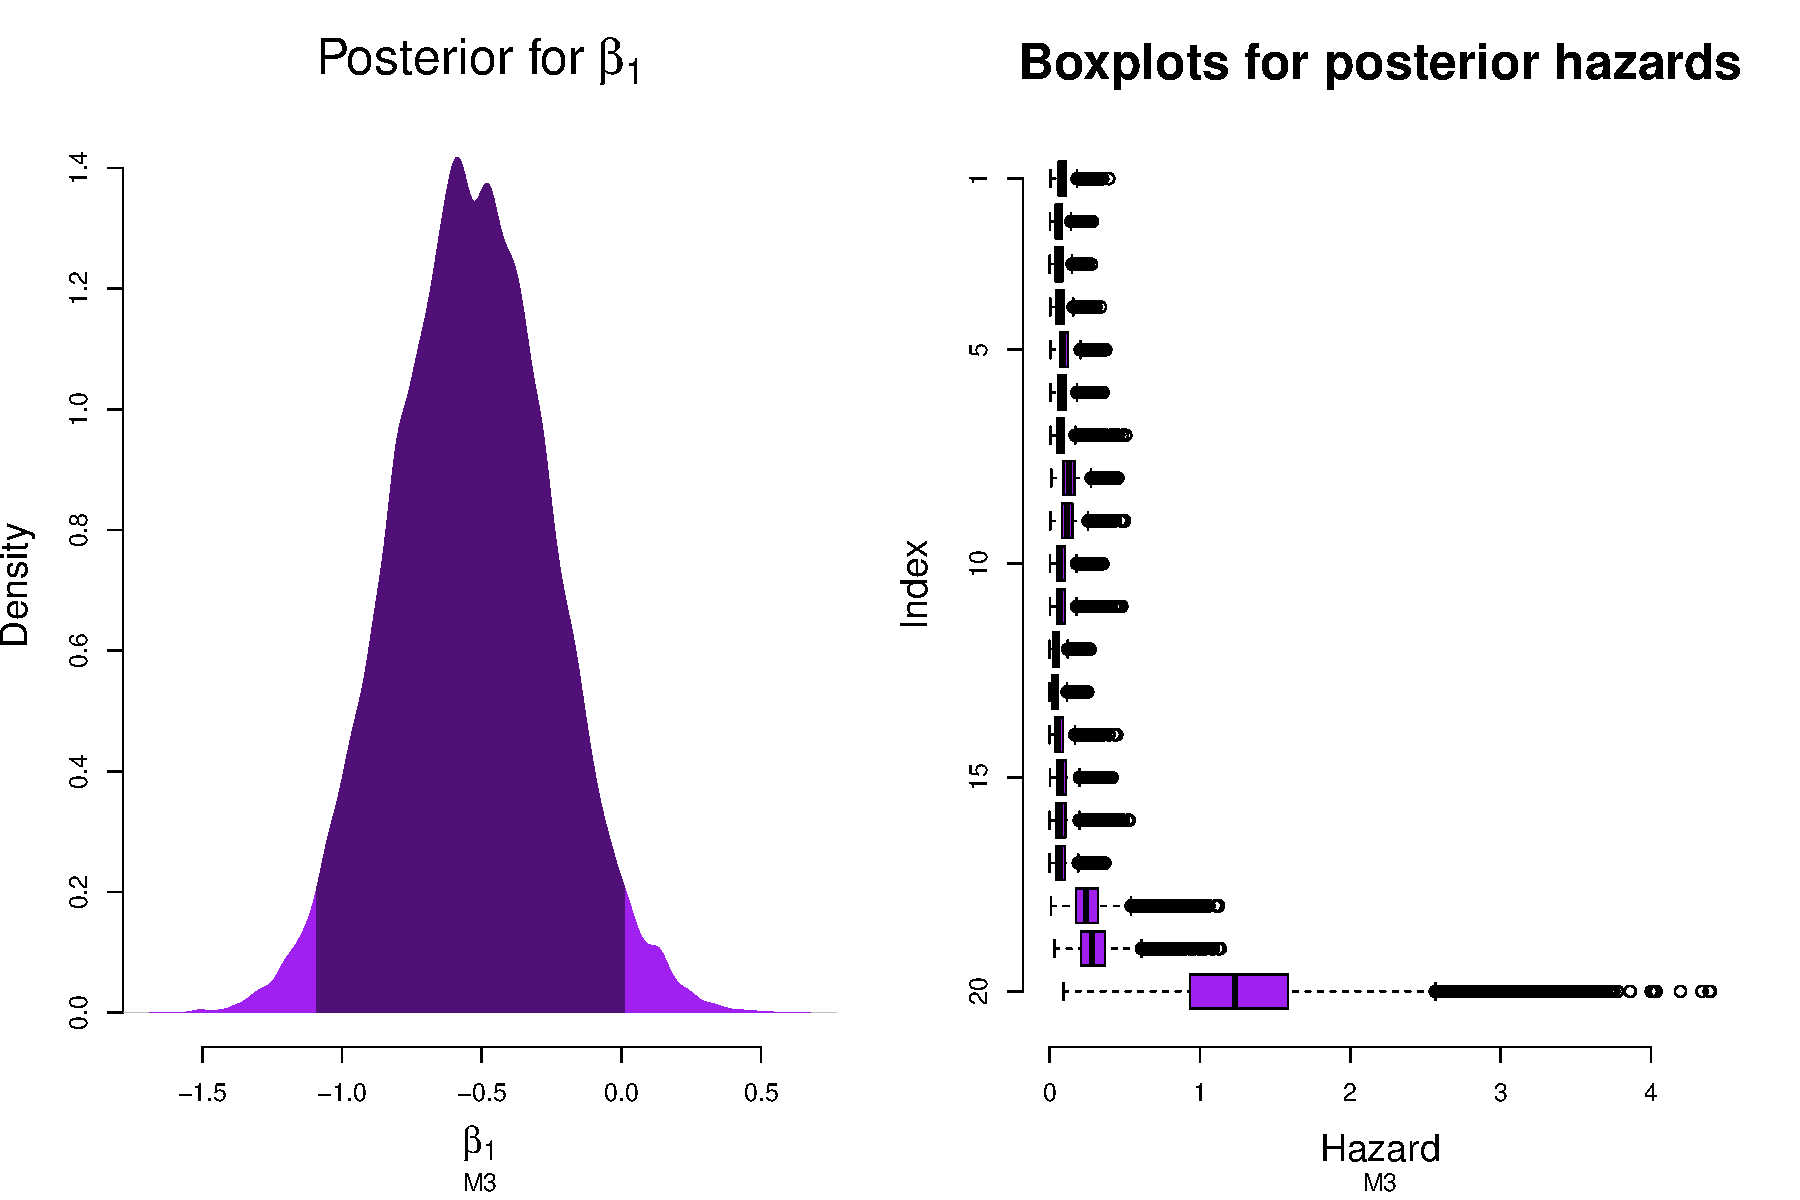
\includegraphics[scale=0.60]{figs/m3_post.pdf}
\bigskip
\bigskip

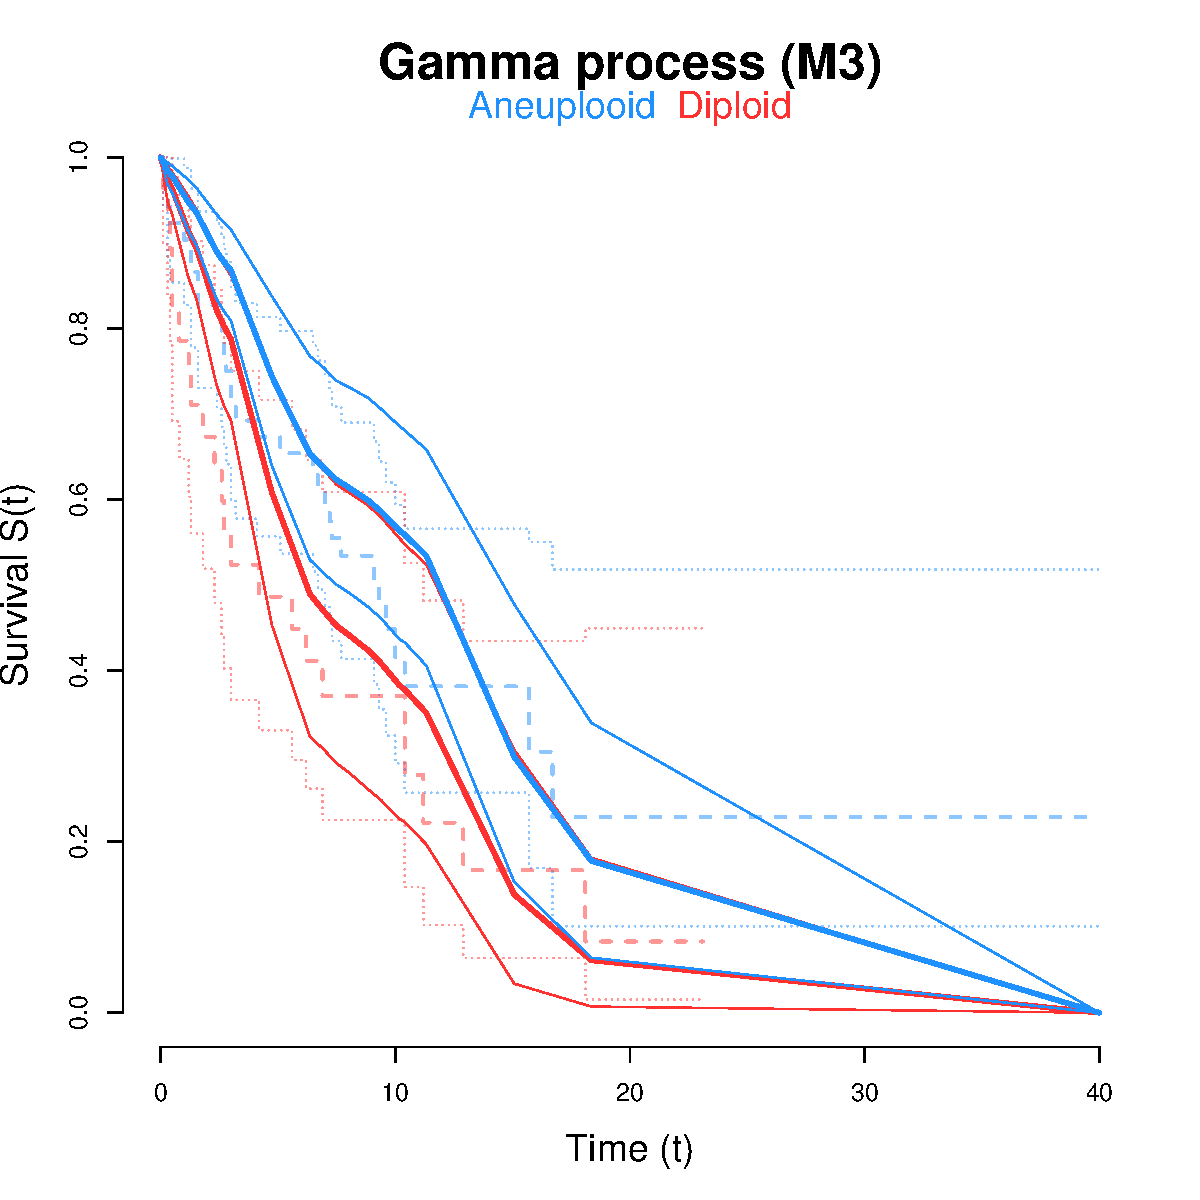
\includegraphics[scale=0.45]{figs/m3_surv.pdf}
\end{center}


\end{document}
